\documentclass[12pt,a4paper]{article}

% incluyendo paquetes
\usepackage[utf8]{inputenc}
\usepackage[spanish]{babel}
\usepackage[acronym]{glossaries}
\usepackage[table]{xcolor}
\usepackage{milibreria}
\usepackage{placeins}

\newcommand{\dpsec}{Dirección de Proyección Social y Extensión Cultural}
\newcommand{\genseg}{Genseg}
\makeglossaries
\newacronym{dpsec}{DPSEC}{Dirección de Proyección Social y Extensión Cultural}
\newacronym{dr}{Dr.}{Doctor}
\newacronym{etc}{etc.}{et cetera}
\newacronym{ieee}{IEEE}{Instituto de Ingenieros Eléctricos y Electrónicos}
\newacronym{ers}{ERS}{especificación de requisitos software}
\newacronym{genseg}{GENSEG}{Gestor de Planes y Proyectos de la Direccion de Proyeccion Social y Extension Cultural}
\newacronym{xp}{XP}{Extreme Programming}

%\graphicspath{{C:/Users/david/imagesppt}} %\incluye todos las imágenes de esa ruta
%\graphicspath{{D:/proyectos_latex/7mo_semestre/gestion_redes/informe_de_redes/main/images}}
\begin{document} % inicio  de documento 

%

\begin{titlepage}
    %\begin{tikzpicture}[overlay, remember picture]
    %    \fill[red] (10cm,-10cm) rectangle (5cm,-15cm);
    %\end{tikzpicture}
    
    \miRectangulo{-2cm}{-4cm}{2cm}{5cm}{rosado}
%   \miRectangulo{x     }{y }{x1    }{y1   }{color}
    
    \miRectangulo{-1.5cm}{-2cm}{-1.2cm}{23.5cm}{black} % 1
    \miRectangulo{-1.8cm}{23.5cm}{5.7cm}{23.2cm}{black} % 2
    \miRectangulo{5.025cm}{23.5cm}{5.33cm}{20cm}{black} % 3
    \miRectangulo{-2.7cm}{-1.7cm}{4.7cm}{-2cm}{black} % 4
    \miRectangulo{4.2cm}{-2cm}{4.5cm}{10cm}{black} % 5

    \begin{textblock}{100}(100,20)
        \begin{flushright}
        {\huge{\textbf{Universidad Nacional del Altiplano}}}\\
        {\normalsize{\textbf{Educando mentes, Cambiando el mundo}}}
        \end{flushright}
        
    \end{textblock}
    
    \begin{tikzpicture}[remember picture, overlay]
        \node at (current page.north west) [anchor=north west, xshift=120mm, yshift=-47mm] {\includegraphics[width=0.45\textwidth]{\logoleft}};
    \end{tikzpicture}

    \begin{textblock}{100}(100,130)
        \begin{flushright}
            {\Large{\textbf{Dirección de Proyección Social y Cultural }}}\\[10pt]
            %{\large{\textbf{Vise Rectorado Académico}}}
        \end{flushright}
    \end{textblock}

    \begin{textblock}{200}(10,163)
        \begin{center}
            
            %\textcolor{azul}{\rule{\linewidth}{0.80mm}}
            % titulo del articulo
            {\LARGE {\textbf{ Especificación de los requisitos del Sistema }}} \par

            \textcolor{azul}{\rule{0.5\linewidth}{0.80mm}} \par
            \vspace{8mm}
            {\large{\textbf{ Sistema de recopilación de información de la \gls{dpsec}}}} \\[10pt]
            {\large{\textbf{\textcolor{azul}{Dr. Milder Zanabria Ortega }}}} \\[20pt]
            {\large{\textbf{Encargados}}}\\[10pt]
            {\large{\textbf{$\looparrowright$   Larota Pilco David Brahyan  $\looparrowleft$ }}}\\[5pt]
            {\large{\textbf{$\looparrowright$    Ronaldo Canaza Flores $\looparrowleft$ }}}\\[5pt]
            {\large{\textbf{$\looparrowright$    Elver Quispe Centeno $\looparrowleft$ }}}\\[5pt]
            %{\large{\textbf{$\looparrowright$  $\mathfrak{David\ Brahyan\ Larota\ Pilco}$   $\looparrowleft$ }}}\\[20pt]
            \today

        \end{center}
    \end{textblock}
    \begin{tikzpicture}[remember picture, overlay]
        \node at (current page.north west) [anchor=north west, xshift=148mm, yshift=-230mm] {\includegraphics[width=0.25\textwidth]{images/QR.png}};
    \end{tikzpicture}

    \begin{textblock}{100}(100,270)
        \begin{flushright}

        {\normalsize{\textbf{QR del respositorio del Proyecto}}}
        \end{flushright}
        
    \end{textblock}
\end{titlepage}


%\begin{titlepage}
%    %\begin{tikzpicture}[overlay, remember picture]
%    %    \fill[red] (10cm,-10cm) rectangle (5cm,-15cm);
%    %\end{tikzpicture}
%    
%    \miRectangulo{-2cm}{-4cm}{2cm}{5cm}{rosado}
%%   \miRectangulo{x     }{y }{x1    }{y1   }{color}
%    
%    \miRectangulo{-1.5cm}{-2cm}{-1.2cm}{23.5cm}{black} % 1
%    \miRectangulo{-1.8cm}{23.5cm}{5.7cm}{23.2cm}{black} % 2
%    \miRectangulo{5.025cm}{23.5cm}{5.33cm}{20cm}{black} % 3
%    \miRectangulo{-2.7cm}{-1.7cm}{4.7cm}{-2cm}{black} % 4
%    \miRectangulo{4.2cm}{-2cm}{4.5cm}{10cm}{black} % 5
%
%    \begin{textblock}{100}(100,20)
%        \begin{flushright}
%        {\huge{\textbf{Universidad Nacional del Altiplano}}}\\
%        {\normalsize{\textbf{Educando mentes, Cambiando el mundo}}}
%        \end{flushright}
%        
%    \end{textblock}
%    
%    \begin{tikzpicture}[remember picture, overlay]
%        \node at (current page.north west) [anchor=north west, xshift=120mm, yshift=-47mm] {\includegraphics[width=0.45\textwidth]{\logoright}};
%    \end{tikzpicture}
%
%    \begin{textblock}{100}(100,130)
%        \begin{flushright}
%            {\Large{\textbf{Dirección de Proyección Social y Cultural }}}\\[10pt]
%            %{\large{\textbf{Vise Rectorado Académico}}}
%        \end{flushright}
%    \end{textblock}
%
%    \begin{textblock}{200}(10,163)
%        \begin{center}
%            
%            %\textcolor{azul}{\rule{\linewidth}{0.80mm}}
%            % titulo del articulo
%            {\LARGE {\textbf{ Especificación de los requisitos del Sistema }}} \par
%
%            \textcolor{azul}{\rule{0.5\linewidth}{0.80mm}} \par
%            \vspace{8mm}
%            {\large{\textbf{ Sistema de recopilación de información de la \gls{dpsec}}}} \\[10pt]
%            {\large{\textbf{\textcolor{azul}{Dr. Milder Zanabria Ortega }}}} \\[20pt]
%            {\large{\textbf{Encargados}}}\\[10pt]
%            {\large{\textbf{$\looparrowright$   Larota Pilco David Brahyan  $\looparrowleft$ }}}\\[5pt]
%            {\large{\textbf{$\looparrowright$    Ronaldo Canaza Flores $\looparrowleft$ }}}\\[5pt]
%            {\large{\textbf{$\looparrowright$    Elver Quispe Centeno $\looparrowleft$ }}}\\[5pt]
%            %{\large{\textbf{$\looparrowright$  $\mathfrak{David\ Brahyan\ Larota\ Pilco}$   $\looparrowleft$ }}}\\[20pt]
%            \today
%
%        \end{center}
%    \end{textblock}
%    \begin{tikzpicture}[remember picture, overlay]
%        \node at (current page.north west) [anchor=north west, xshift=148mm, yshift=-230mm] {\includegraphics[width=0.25\textwidth]{images/QR.png}};
%    \end{tikzpicture}
%
%    \begin{textblock}{100}(100,270)
%        \begin{flushright}
%
%        {\normalsize{\textbf{QR del respositorio del Proyecto}}}
%        \end{flushright}
%        
%    \end{textblock}
%\end{titlepage}
%%//--------------------------------------
%@article{prueba,
%  title={prueba del documento lenguaje Latex},
%  author={Autor},
%  journal={https://www.overleaf.com/},
%  volume={13},
%  number={36},
%  pages={34--36},
%  year={2022}
%}
%
%
%\begin{figure}[h]
%    \centering
%    \includegraphics[width=0.5\textwidth]{images/medicion_con_tacometro.png}
%    \caption{se realizo la medición con el tacómetro} 
%\end{figure}
%
%\begin{tabular}{ l c l }
%Tipo  			& = & 	GL-90L-4B5 \\
%Ip              & = &	55 \\
%Cos  $\varphi$    & = &  	  0.78 \\
%Voltaje         & = &	 230/400V \\
%Potencia	    & = &	2HP \\
%Intensidad    	& = & 	6.1/3.5 \\
%Frecuencia  	& = & 	60HZ \\
%Rpm     		& = &	1680 
%\end{tabular} % incluyendo la caratula
\usetikzlibrary{calc}
\begin{titlepage}
    \centering
    \miRectangulo{-3.2cm}{10cm}{13.7cm}{4.9cm}{azulm}{0}
    \miRectangulo{0cm}{7.5cm}{9cm}{6cm}{azulm}{45}
    \miRectangulo{-4cm}{-15cm}{15cm}{6cm}{azulm}{0}

    \miRectangulo{-16cm}{-7cm}{10cm}{6cm}{azulm}{45}
    \miRectangulo{-11cm}{-15cm}{9cm}{3cm}{azulm}{0}
    \miRectangulo{-5cm}{-4.5cm}{3.5cm}{3.5cm}{azulm}{45}
    \begin{figure}[h]
        \miRomboImagen{-2.3}{-10.5}{images/magno.jpeg}{20}
    \end{figure}
    
    \begin{textblock}{70}(135,13)
        \begin{flushright}
            {\large{\textcolor{white}{Dirección de Proyección Social y Extensión Cultural}}}\\
            %{\normalsize{\textcolor{white}{Educando mentes, Cambiando el mundo}}}
        \end{flushright} 
    \end{textblock}
    \begin{tikzpicture}[remember picture, overlay]
        \node at (current page.north west) [anchor=north west, xshift=90mm, yshift=-2mm] {
\includegraphics[width=0.25\textwidth]{images/logodpsecsf.png}};
    \end{tikzpicture}

    \begin{textblock}{100}(100,60)
        \begin{flushright}
            {\Huge{\textbf{2024}}}\\[20pt]
            {\fontsize{50}{60}\selectfont\textbf{\MakeUppercase{\genseg}}}\\[20pt]
            {\large{\textbf{Gestor de Proyectos de la Dirección de Proyección Social y Extensión Cultural}}}\\[15pt]
            {\Large{\textbf{Documento de Propuesta de Desarrollo}}}\\[15pt]
        \end{flushright} 
    \end{textblock}

    \begin{textblock}{100}(120,140)
        \textcolor{azulm}{\rule{0.5\linewidth}{0.90mm}} \par
    \end{textblock}
    
    \begin{textblock}{100}(100,160)
        \begin{flushright}
            {\large{\textbf{Fecha: \\[10pt] \today}}}\\[15pt]
            {\large{\textbf{ Propuesto por: }}}\\[5pt]
            {\large{\textbf{ Larota Pilco David Bahyan }}}\\[5pt]
            {\large{\textbf{ Pari Choquehuanca Bernardo }}}\\[5pt]
            {\large{\textbf{ Quispe Bravo Marco Alexander }}}\\[5pt]
            {\large{\textbf{ Chura Cutipa Lenin Alonso }}}\\[5pt]
            %{\large{\textbf{ Apaza Ccapa Rosmery }}}\\[5pt]
        \end{flushright} 
    \end{textblock}

    \begin{textblock}{100}(100,256)
        \begin{flushright}
            {\huge{\textcolor{white}{Universidad Nacional del Altiplano}}}\\
            {\normalsize{\textcolor{white}{Educando mentes, Cambiando el mundo}}}
        
        \end{flushright} 
    \end{textblock}
    \begin{tikzpicture}[remember picture, overlay]
        \node at (current page.north west) [anchor=north west, xshift=50mm, yshift=-250mm] {
\includegraphics[width=0.25\textwidth]{images/qr_code.png}};
    \end{tikzpicture}

\end{titlepage}
\tableofcontents % índice automático
% Índice de figuras
\listoffigures

% Índice de tablas
\listoftables
\pagestyle{fancy} \mystyle \newpage % Aplicar el estilo de encabezado y pie de página
% inicio del documento




\section{Introducción }
Este plan de Desarrollo de software es una versión preliminar preparada para ser incluida 
en la propuesta elaborada como respuesta el proyecto \textquotedblleft(\gls{dpsec})\textquotedblright \ Este documento
provee una visión global del enfoque de desarrollo propuesto.
\espacio
En el proyecto se usa una metodologia \textbf{\gls{xp}} en la que únicamente
se procederá a cumplir con las fases: \textbf{planificación, diseño, codificación, pruebas y lanzamiento.}
que marca la metodologia de desarrollo de software \gls{xp}.
Se incluirá el detalle para las fases de Análisis, Diseño, Desarrollo e Implementación.
del sistema propuesto para la gestion de proyectos y planes.
\espacio
El enfoque de desarrollo propuesto constituye una configuración del proceso
de gestion de proyectos y planes dentro de la \gls{dpsec} de acuerdo a las 
caracteristicas del proyecto \gls{genseg}. 

\subsection{Propósito } 
Este es el Cambio de Berning
\subsection{Alcance}
 
\subsection{Justificación/Resumen}


\section{Personal involucrado}

\begin{table}[h!]
    \centering
    \begin{tabular}{|p{7cm}|p{8cm}|}
    \hline
    \rowcolor{pastelBlue} \textbf{Nombre} & David Brahyan Larota Pilco \\ \hline
    \textbf{Rol} & Analista, diseñador y programador \\ \hline
    \rowcolor{pastelBlue} \textbf{Categoría profesional} & Ingeniería de sistemas \\ \hline
    \textbf{Responsabilidad} & Análisis de información y diseño \\ \hline
    \rowcolor{pastelBlue} \textbf{Información de contacto} & \href{mailto:dlarotap@est.unap.edu.pe}{\textbf{dlarotap@est.unap.edu.pe *}} \\ \hline
    \end{tabular}
    \caption{Tabla de información personal}
    \label{tab:personal_info}
\end{table}




\section{Ámbito del Sistema}
\textbf{Nombre del sistema:} Sistema de recopilación de información en los proyectos de la \gls{dpsec}.
\espacio 
El sistema recopila información estructurada de las actividades, planes y proyectos de los programas de estudio (44 programas de estudio).

\espacio 
Los principales beneficios en la reducción de papel, articulación con los programas de estudio, logro de indicadores institucionales y administrativos información en tiempo real oportuna procesos eficientes justo a tiempo.

\subsection*{Las Metas principales son:}
\begin{itemize}
    \item Cobertura de 44 programas de estudio.
    \item La dirección DPSEC y las subunidades.
    \item Satisfacer a los 132 usuarios del sistema.
    \item abarcar documentos estructurados como proyectos y planes.
    
    \end{itemize}
    
    
    \subsection*{Objetivo general }
    recopilar requisitos que tengan la información para que permita implementar el sistema de Recopilación de Datos.
    
    
    \section{Definiciones, Acrónimos y Abreviaturas}
    \subsection*{Definición}
    \Dbox{Title}{hola a todos asmldnksjahnd jsahdklsa hdlsa hldhsajdskñaj }

    \printglossaries

    
    \section{Resumen }

El resumen de las 4 etapas

\begin{figure}[!htbp]
    \centering
    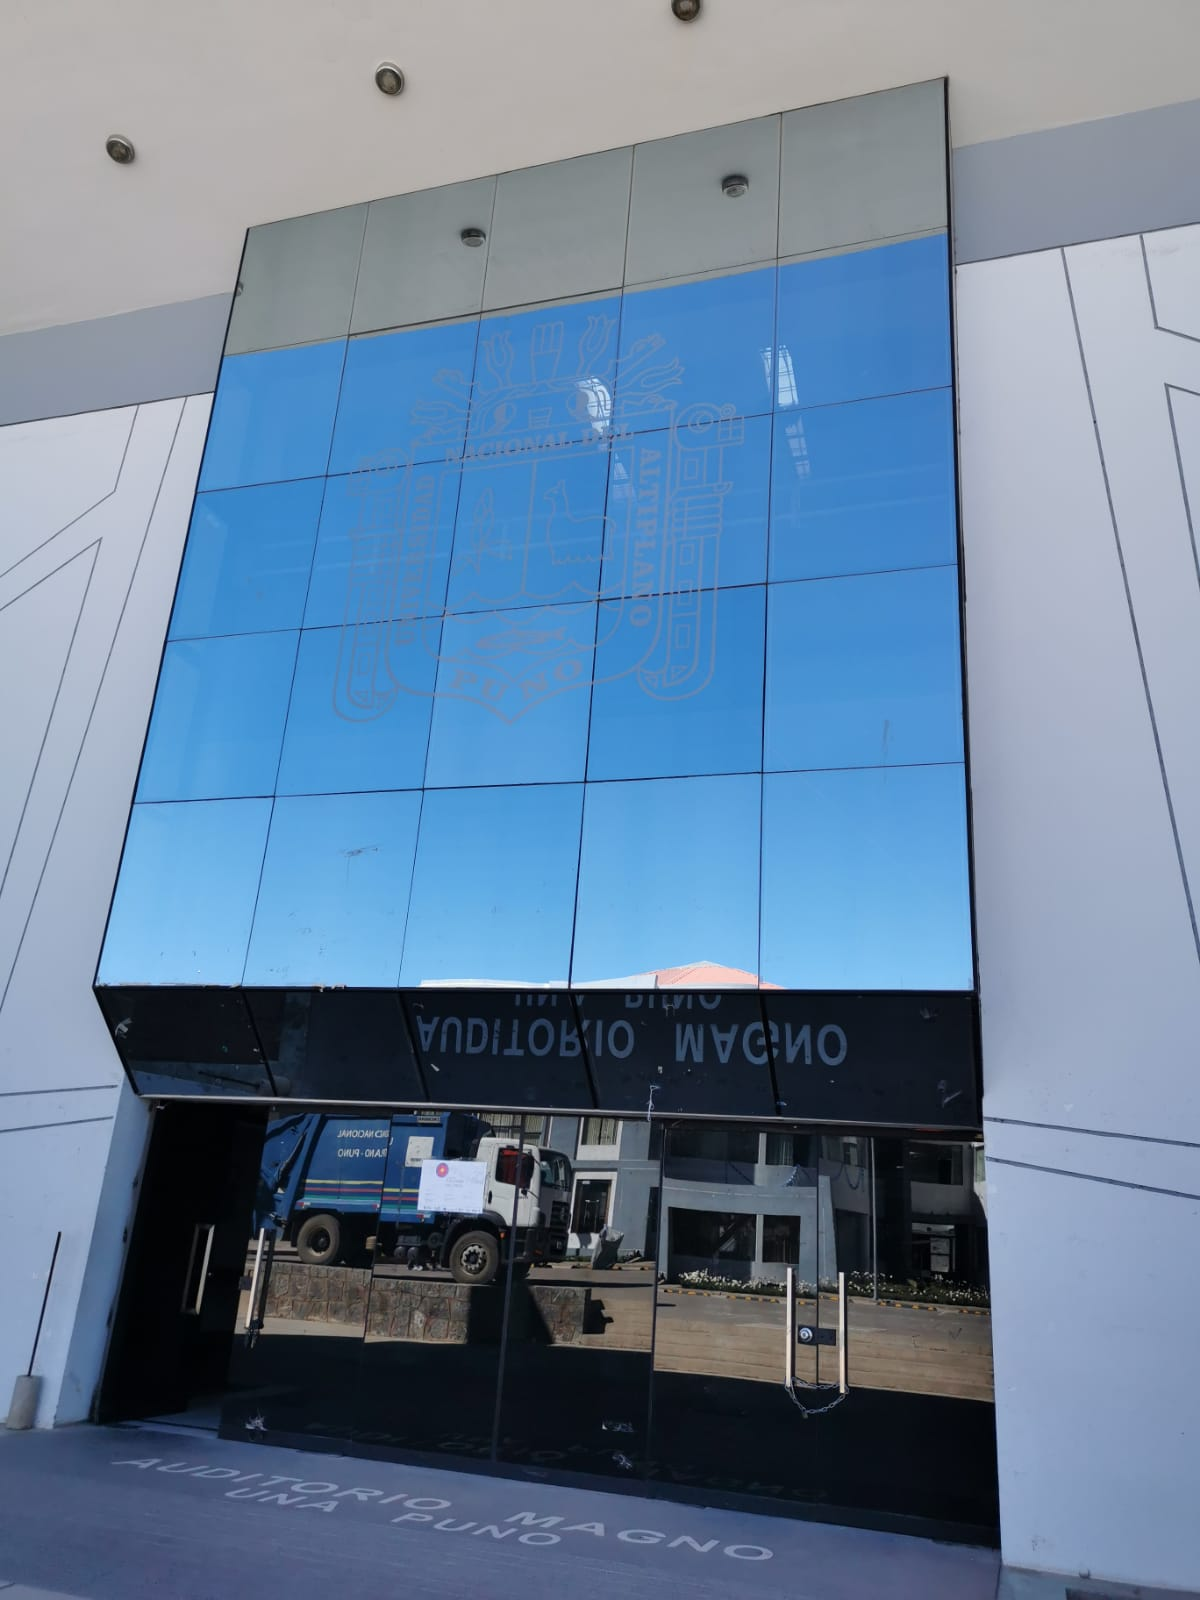
\includegraphics[width=0.7\textwidth]{images/magno.jpeg}
    \caption{Descripción de la imagen}
    \label{fig:miImagen}
\end{figure}
\FloatBarrier
\section{asdsa}

adasdsad mirando la tabla [tab:\ref{tab:personal_info}]
\shortcite{audit_operativa}
    \begin{comment}
    usuario
\subsubsection*{Administrador} Un super administrador que administre a otro administrador, roles por facultad.
\subsubsection*{Requisito funcional} Recopilar documento, información sobre un plan de trabajo de las 44 carreras y 3 subunidades.
\subsubsection*{Requisito no funcional} Si se quita un rol a una unidad, se quitará para todos sin excepción .


\subsection*{Acrónimos}
\begin{table}[!htbp]
    \centering
    \caption{Acrónimos}
    \label{tb:acronimos}
    \begin{tabular}{cl}
        \toprule
        \textbf{Acronimo} & \textbf{Significado} \\
        \midrule
        ERS & Especificación de requisitos de Software. \\
        UML & Lenguaje de Modelo Unificado. \\
        API & Interfaz de Programación de Aplicaciones. \\
        DPSEC & Dirección de Proyección Social y Extensión Cultural. \\
        IEEE & Práctica recomendada para especificaciones de requisitos de software. \\
        Administrador & Persona que usará el sistema para definir roles de otros administradores de menor Jerarquía. \\
        RFA & Requerimiento Funcional Administrativo.  \\

        \bottomrule
    \end{tabular}
\end{table}


\subsection*{Abreviaturas}
El \gls{dr} Smith es un destacado investigador en su campo. La lista incluye manzanas, peras, \gls{etc}.

\printglossaries
\end{comment}


\newpage
\section{Referencias}
\bibliographystyle{apacite}
\bibliography{referencias.bib}


\end{document}